\documentclass{beamer}

\usepackage[utf8]{inputenc}
\usepackage[brazil]{babel}
\usepackage{graphicx,hyperref,icmc,url}
\usepackage{subcaption}
\usepackage{multirow}
\usepackage{minted}
\usepackage{tikz}
\usepackage{array}
\usepackage{listings}% http://ctan.org/pkg/listings
\newcommand{\destaq}[1]{\textcolor{purple}{\textbf{#1}}}


% The title of the presentation:
%  - first a short version which is visible at the bottom of each slide;
%  - second the full title shown on the title slide;
\title[Paradigma orientado a objetos]{Paradigma orientado a objetos}

% Optional: a subtitle to be displayed on the title slide


% The author(s) of the presentation:
%  - again first a short version to be displayed at the bottom;
%  - next the full list of authors, which may include contact information;
\author[André, Eduardo, Gustavo, Matheus, Thiago]{
André Luís Mendes Fakhoury\\ Eduardo Dias Pennone\\ Gustavo Vinícius Vieira Silva Soares\\ Matheus Steigenberg Populim\\ Thiago Preischadt Pinheiro\\ \bigskip
\textsc{SCC0217 - Linguagens de Programação e Compiladores}\\
Prof. Diego Raphael Amancio
}

% \\ \bigskip
    % \large{}

% The institute:
%  - to start the name of the university as displayed on the top of each slide
%    this can be adjusted such that you can also create a Dutch version
%  - next the institute information as displayed on the title slide
\institute[ICMC/USP]{ICMC - USP}

% Add a date and possibly the name of the event to the slides
%  - again first a short version to be shown at the bottom of each slide
%  - second the full date and event name for the title slide
\date[2021]{\footnotesize{1 de julho de 2021}}

\AtBeginSection[]
{
    \begin{frame}<beamer>{Sumário}
        \tableofcontents[currentsection]
    \end{frame}
}

\begin{document}
    
    \begin{frame}[plain]
        \titlepage
    \end{frame}
    
    \begin{frame}
      \frametitle{Sumário}
      \tableofcontents
    \end{frame}
    
%%%%%%%%%%%%%%%%%%%%%%%%%%%%%%%%%%%%%%%%%%%%%%%%%%%%%%%%%%%%%%%%

\section{Introdução}

\begin{frame}{Introdução}
\framesubtitle{Histórico}
\begin{itemize}
    \item O conceito de programação orientada a objetos teve suas raízes no SIMULA 67, mas não foi totalmente desenvolvido até que a evolução do Smalltalk resultou no Smalltalk 80. 
    \item Muitos consideram o Smalltalk como sendo o modelo básico para uma linguagem de programação puramente orientada a objetos.
\end{itemize} 
\end{frame}

\begin{frame}{Introdução}
\framesubtitle{O paradigma da orientação a objetos}
\begin{itemize}
    \item Uma linguagem orientada a objetos deve fornecer suporte para três recursos-chave da linguagem: tipos de dados abstratos, herança e vinculação dinâmica de chamadas de método a métodos.
    \item Com base nesses recursos temos os 4 pilares da orientação a objetos: Abstração, Encapsulamento, Herança e Polimorfismo.
\end{itemize} 
\end{frame}

\section{Conceitos importantes presentes no paradigma}

\begin{frame}{Conceitos importantes presentes no paradigma}
\framesubtitle{Classe}
\begin{itemize}
    \item Uma abstração de um conjunto de objetos que possuem características em comum.
    \item A descrição de propriedades, estados, comportamentos e ações de um conjunto de objetos.
\end{itemize} 
\end{frame}

\begin{frame}{Conceitos importantes presentes no paradigma}
\framesubtitle{Objeto}
\begin{itemize}
    \item A instância de uma classe.
    \item Representação de um objeto do mundo real pertencente a uma classe especificada.
    \item Caracterizado por atributos e métodos.
\end{itemize} 
\end{frame}

\begin{frame}{Conceitos importantes presentes no paradigma}
\framesubtitle{Atributos}
\begin{itemize}
    \item As características, propriedades ou estados de um objeto.
    \item Exemplos: tamanho, cor, peso. 
\end{itemize} 
\end{frame}

\begin{frame}{Conceitos importantes presentes no paradigma}
\framesubtitle{Métodos}
\begin{itemize}
    \item Os comportamentos, ações ou funcionalidades que um objeto pode desempenhar.
    \item Exemplos: comer, voar, latir.
\end{itemize} 
\end{frame}

\begin{frame}{Conceitos importantes presentes no paradigma}
\framesubtitle{Abstração}
\begin{itemize}
    \item Uma abstração é uma visão ou representação de uma entidade que inclui apenas os atributos mais significativos. Em um sentido geral, a abstração permite coletar instâncias de entidades em grupos nos quais seus atributos comuns não precisam ser considerados.
\end{itemize} 
\end{frame}

\begin{frame}{Conceitos importantes presentes no paradigma}
\framesubtitle{Herança}
\begin{itemize}
    \item A herança possibilita que as classes compartilhem seus métodos e atributos entre si seguindo uma hierarquia baseada nos níveis de abstração.
    \item Facilitam a reutilização do código, uma vez que atributos e métodos das classes superiores podem ser aproveitados.
\end{itemize} 
\end{frame}

\begin{frame}{Conceitos importantes presentes no paradigma}
\framesubtitle{Encapsulamento}
\begin{itemize}
    \item Controla o acesso à atributos e métodos de uma classe.
    \item Evitar o acesso direto a propriedade do objeto adiciona segurança à aplicação.
    \item O código pode evoluir a partir de uma interface em comum.
\end{itemize} 
\end{frame}

\begin{frame}{Conceitos importantes presentes no paradigma}
\framesubtitle{Polimorfismo}
\begin{itemize}
    \item Consiste na alteração do funcionamento interno de um método herdado de um objeto pai.
    \item Subclasses diferentes que possuem uma mesma classe pai, possuem comportamentos diferentes em relação ao mesmo método herdado.
\end{itemize} 
\end{frame}

\section{Herança, encapsulamento e polimorfismo}

\begin{frame}{Herança}
\framesubtitle{}
\begin{itemize}
    \item Criar uma classe derivada a partir de uma classe base
    \item Classe derivada herda os atributos e métodos da base
\end{itemize}
\end{frame}

\begin{frame}{Herança}
\framesubtitle{}
\begin{itemize}
    \item Normalmente os construtores e destrutores não são herdados
    \item Métodos herdados podem ser sobrescritos
    \item Novos métodos e atributos podem ser adicionados
\end{itemize}
\end{frame}

\begin{frame}{Herança}
\framesubtitle{Tipos}
\begin{itemize}
    \item Simples
    \item Múltipla
    \item Multinível
\end{itemize}
\end{frame}

\begin{frame}{Herança}
\framesubtitle{Simples}
\begin{itemize}
    \item Cada classe tem no máximo uma superclasse
    \item A hierarquia pode ser representada por uma árvore
\end{itemize}
\begin{figure}
	
\includegraphics{img/simples}
\end{figure}
\end{frame}

\begin{frame}{Herança}
\framesubtitle{Múltipla}
\begin{itemize}
    \item Cada classe pode ter diversas superclasses
    \item Pode ser necessário tratar ambiguidades na herança
    \item A hierarquia pode ser representada por um grafo direcionado
\end{itemize}
\begin{figure}
	
\includegraphics{img/multipla.png}
\end{figure}
\end{frame}

\begin{frame}{Herança}
\framesubtitle{Multinível}
\begin{itemize}
    \item Uma classe derivada pode ser base de outra classe
\end{itemize}
\begin{figure}
	
\includegraphics{img/multinivel.png}
\end{figure}
\end{frame}

\begin{frame}{Herança}
\framesubtitle{Usos}
\begin{itemize}
    \item Reuso de código
    \item Implementar uma mesma interface de diferentes formas
\end{itemize}
\end{frame}

\begin{frame}{Encapsulamento}
\framesubtitle{}
\begin{itemize}
    \item Agrupar dados e métodos que agem sobre esses dados
    \item Restringir o acesso direto aos dados
\end{itemize}
\end{frame}

\begin{frame}{Encapsulamento}
\framesubtitle{Usos}
\begin{itemize}
    \item Esconder informação
    \item Esconder detalhes de implementação
    \item Evitar que o objeto entre em um estado inválido
\end{itemize}
\end{frame}

\begin{frame}{Polimorfismo}
\framesubtitle{}
\begin{itemize}
    \item Utilizar o mesmo símbolo para representar vários tipos
    \item Tratar objetos de uma classe derivada com objetos da classe base
\end{itemize}
\end{frame}

\begin{frame}{Polimorfismo}
\framesubtitle{Tipos}
\begin{itemize}
    \item Ad hoc
    \item Paramétrico
    \item Por subtipos
\end{itemize}
\end{frame}

\begin{frame}[fragile]
\frametitle{Polimorfismo}
\framesubtitle{Ad hoc}
\begin{itemize}
    \item Sobrecarga de operador/função
    \item Definir diversas funções com mesmo nome e quantidade de argumentos, mas com diferentes tipos
\end{itemize}
\begin{verbatim}
    soma(a: int, b: int) : int
    soma(a: float, b: float) : float
\end{verbatim}
\end{frame}

\begin{frame}{Polimorfismo}
\framesubtitle{Paramétrico}
\begin{itemize}
    \item Definir funções que aceita um tipo genérico
    \item O comportamento da função é uniforme em relação ao tipo da entrada
\end{itemize}
\end{frame}

\begin{frame}{Polimorfismo}
\framesubtitle{Por subtipos}
\begin{itemize}
    \item Definir uma função que aceita um tipo A
    \item A função funciona corretamente para um subtipo de A
\end{itemize}
\end{frame}

\section{Tipagem dinâmica e estática}

\begin{frame}{Tipagem dinâmica e estática}
\framesubtitle{Escolha de design}
\begin{itemize}
    \item No paradigma orientado a objetos, as linguagens possuem uma escolha com relação à tipagem: dinâmica ou estática
    \item Equilíbrio entre o custo de execução e de compilação
    \item Algumas linguagens de orientação a objetos realizam vínculo estático ou dinâmico a depender de algumas condições específicas
\end{itemize} 
\end{frame}

\begin{frame}[fragile]{Tipagem dinâmica}
\begin{itemize}
    \item Muitas vezes, chamadas internas a métodos implementados por subclasses possuem uma informação incompleta
    \item Em Java, por exemplo, há diversas implementações do método add em classes diferentes.
\end{itemize}
\begin{verbatim}
        this.add(elemento);
\end{verbatim}
\end{frame}

\begin{frame}[fragile]{Tipagem dinâmica}
\begin{itemize}
    \item Muito comum para situações de polimorfismo
    \item Uma referência pode apontar para objetos de classes distintas
    \item O sistema precisa determinar, em tempo de execução, a qual classe um método se refere, visto que há ambiguidade
    \item Provê facilidade no desenvolvimento e manutenção dos objetos da aplicação
\end{itemize}
\end{frame}


\begin{frame}[fragile]{Tipagem estática}
\begin{itemize}
    \item Muitas vezes um custo de execução pode ser convertido em compilação
    \item A informação completa ou restrição do contexto permite essa conversão
    \item Em Java, por exemplo, quando não há dúvidas da origem de uma chamada de um método, o compilador armazena as informações dos métodos e classes utilizadas
\end{itemize}
\begin{verbatim}
        colecao.addAll(outraColecao);
\end{verbatim}
\begin{itemize}
    \item A classe precisa implementar AbstractCollection, e portanto o método addAll deve ser definido como static ou final
\end{itemize}
\end{frame}

\section{Exemplos de linguagens}

\subsection{Smalltalk}

\begin{frame}{Smalltalk}
\framesubtitle{Histórico}
    \begin{itemize}
        \item Teve inicio com um projeto de pesquisa na Xerox Corporation's Palto Alto Research Center em 1970
        \item Foi continuado por Adele Goldberg e Daniel Ingalls
        \item Influência de Simula e Lisp
        \item Foi inovadora para a divisória criada para interfaces gráficas.
        \item Ambiente de desenvolvimento completo, com sistemas de janelas, menus e cursor
    \end{itemize}
\end{frame}

\begin{frame}{Smalltalk}
\framesubtitle{Design}
    \begin{itemize}
        \item Puramente orientada a objetos (até constantes)
        \item Mensagens e Objetos de dados
        \item Objetos possuem características e comportamentos
    \end{itemize}
\end{frame}

\begin{frame}[fragile]{Smalltalk}
\framesubtitle{Design}
    \begin{itemize}
        \item Características são atributos de uma classe ou instância
        \item Comportamentos são ações a serem reproduzidas por métodos
        \item Métodos podem enviar outras mensagens e podem devolver objetos
        \item Mensagens podem ser unárias ou até mesmo incluir parâmetros
    \end{itemize}
\begin{verbatim}
        Set new includes: 'Hello'
        (Array new: 10) at: 1 put: 66
\end{verbatim}
\end{frame}

\begin{frame}{Smalltalk}
    \begin{figure}
	\centering
	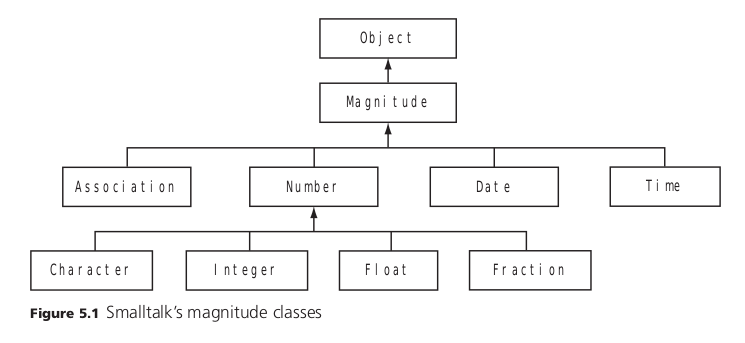
\includegraphics[width=0.8\linewidth]{img/magnitude}
	\caption{Hierarquia de classes de magnitude \cite{louden2012}}
	\label{fig:herancadiamante}
\end{figure}
\end{frame}


\subsection{C++ e Java}

\begin{frame}{C++ e Java}
\framesubtitle{C++ e Java}
\begin{itemize}
    \item Linguagens muito relevantes atualmente muito importantes ao longo da história e no contexto atual de programação
    \item Orientação a objetos como um dos principais fatores de popularidade.

\end{itemize} 
\end{frame}

\begin{frame}{C++ e Java}
\framesubtitle{Popularidade}
    \begin{figure}
    	\centering
    	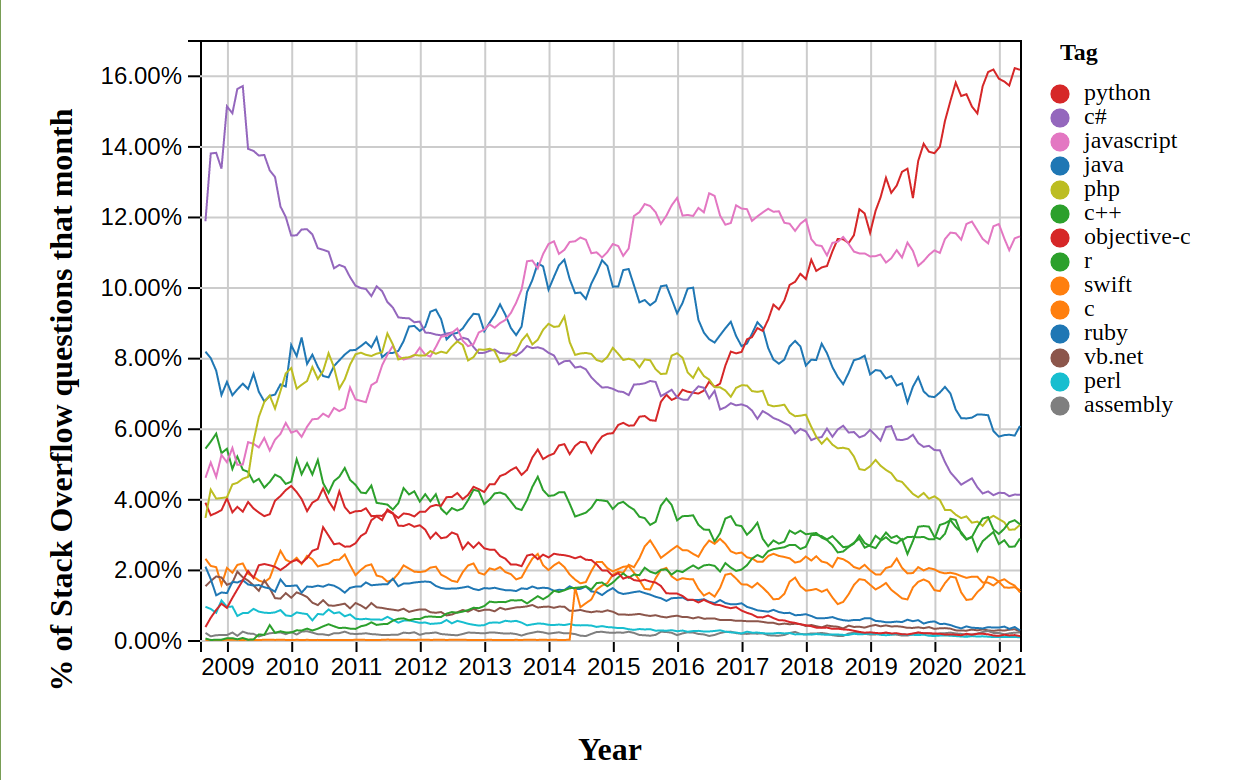
\includegraphics[width=0.9\linewidth]{img/image_pop.png}
    	\caption{Popularidade das linguagens de programação.\cite{stackoverflow}}
    	\label{fig:popularidade}
    \end{figure}
\end{frame}



\begin{frame}{C++ e Java}
\framesubtitle{C++}
\begin{itemize}
    \item Lançada por Bjarne Stroustrup em 1985.
    \item Planejada para ser um "C com classes".
    \item Adotou recursos de diversos paradigmas.
    \item Muito utilizada para contextos com recursos limitados ou que exijam alto desempenho, como software de sistema, embarcados, computação científica, gráficos, jogos,  etc.
\end{itemize} 
\end{frame}


\begin{frame}{C++ e Java}
\framesubtitle{Java}
\begin{itemize}
    \item Lançada pela Sun Microsystems em 1996.
    \item Fortemente orientada a objetos.
    \item Write Once, Run Anywhere (JVM).
    \item Uma das linguagens mais utilizadas atualmente no contexto de finanças, projetos corporativos, desenvolvimento de apps, etc.
\end{itemize} 
\end{frame}


\begin{frame}{C++ e Java}
\framesubtitle{Diferenças }
\begin{itemize}
    \item Ao contrário do C++, Java não suporta sobrecarga de operador ou herança múltipla para classes, embora herança múltipla seja compatível com interfaces.
    \item Gerenciamento de memória: Manual vs Garbage Colector.\cite{OOManagement}
    \item Passagem de argumentos por ponteiros vs por valor.

\end{itemize} 
\end{frame}



\section{Questões de design e implementação}

\begin{frame}
\frametitle{Questões de projeto}
\framesubtitle{Design e implementação}
\begin{itemize}
	\item Algumas questões surgem com o paradigma orientado a objetos
	\item Escolha entre \destaq{flexibilidade} e \destaq{eficiência de execução}
	\item Algumas linguagens focam mais em eficiência que outras
\end{itemize}
\end{frame}

\begin{frame}
\frametitle{Questões de projeto}
\framesubtitle{Exclusividade de Objetos}
\begin{itemize}
	\item Introdução do conceito de classes além dos tipos existentes
	\item \destaq{Vantagens:} uniformidade e elegância
	\item \destaq{Desvantagens:} menor eficiência, pois operações simples são feitas por processos de passsagem de mensagens
\end{itemize}
\end{frame}

\begin{frame}
\frametitle{Questões de projeto}
\framesubtitle{Exclusividade de Objetos}
Escolha entre tipos e classes:
\begin{enumerate}
\item Adição de classes e modelo de objetos à linguagem já existente \texttt{(Objective-C)}
\item Classes são construtores de tipos, ou seja, declarações de classes fazem parte do sistema de tipagem \texttt{(C++)}
\item Exclusão dos outros tipos estruturados, e todos os tipos são classes \texttt{(Smalltalk)}
\end{enumerate}
\end{frame}


\begin{frame}
\frametitle{Questões de projeto}
\framesubtitle{Exclusividade de Objetos}
Exemplos das linguagens:

\begin{itemize}
\item \texttt{Smalltalk}, \texttt{Ruby}: apenas objetos
\item \texttt{C++}, \texttt{Objective-C}, \texttt{Java}, \texttt{C\#}: tipos primitivos + objetos
\end{itemize}
\end{frame}

\begin{frame}
\frametitle{Questões de projeto}
\framesubtitle{Diferenças entre classes e subclasses}

Existem muitas possibilidades de diferenças entre subclasses e classes pai ou base
\begin{itemize}
\item Divergir no número de métodos, parâmetros de algum método, corpo de algum método, tipos de retornos dos métodos diferentes...
\end{itemize}

Normalmente são restringidos:
\begin{itemize}
\item A subclasse restringe-se a um subtipo da classe pai - relacionamentos \destaq{é-um(a)}
\item Métodos da subclasse que sobrescrevem métodos da classe pai devem ser compatíveis com os sobrescritos
\end{itemize}

\end{frame}

\begin{frame}
\frametitle{Questões de projeto}
\framesubtitle{Verificação de tipos e polimorfismo}

Variáveis \destaq{polimórficas} podem referenciar objetos da classe base ou descendentes

\begin{itemize}
	\item Por isso, nem sempre podem ser determinadas estaticamente;
	\item Questão é: sendo dinamicamente, quando realizar as verificações de tipos das vinculações.
\end{itemize}
\end{frame}

\begin{frame}
\frametitle{Questões de projeto}
\framesubtitle{Herança simples e múltipla}

Nas heranças múltiplas, uma nova classe herda duas ou mais classes
\begin{itemize}
	\item Isso pode impactar a linguagem tanto na \destaq{complexidade} de programação quanto na \destaq{eficiência}.
\end{itemize}

\end{frame}

\begin{frame}
\frametitle{Questões de projeto}
\framesubtitle{Herança simples e múltipla}

Exemplo de questão que surge: \destaq{heranças compartilhadas}.

\begin{figure}
	\centering
	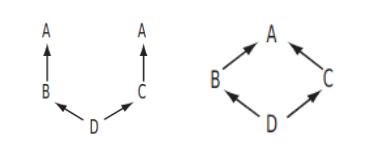
\includegraphics[width=0.7\linewidth]{img/heranca_diamante}
	\caption{A mesma classe pai A é referenciada por B e por C. \cite{louden2012}}
	\label{fig:herancadiamante}
\end{figure}

\begin{itemize}
\item Na esquerda: duas cópias da classe $A$ (herança repetida).
\item Na direita: a mesma cópia de $A$ usada por $B$ e $C$ (herança compartilhada).
\end{itemize}
\end{frame}

\begin{frame}
\frametitle{Questões de projeto}
\framesubtitle{Herança simples e múltipla}
Tipos de herança presentes em algumas linguagens:

\begin{itemize}
	\item \texttt{Smalltalk}: apenas simples
	\item \texttt{Objective-C}: apenas simples, alguns efeitos com protocolos
	\item \texttt{Java}, \texttt{C\#}: apenas simples, alguns efeitos com interfaces
	\item \texttt{Ruby}: apenas simples, alguns efeitos com módulos
	\item \texttt{C++}: ambas
\end{itemize}
\end{frame}

\begin{frame}
\frametitle{Questões de projeto}
\framesubtitle{Vinculação estática e dinâmica}

\begin{itemize}
\item Vinculações estáticas ou dinâmicas;
\item Estáticas são mais rápidas, mas as dinâmicas também possuem vantagens;
\item \destaq{Exemplos em linguagens:}
\item \texttt{Smalltalk}, \texttt{Ruby}: todas as vinculações são dinâmicas
\item \texttt{C++}, \texttt{Objective-C}, \texttt{Java}, \texttt{C\#}: podem ser estáticas ou dinâmicas
\end{itemize}
\end{frame}

\begin{frame}
\frametitle{Questões de projeto}
\framesubtitle{Alocação e liberação de objetos}
\begin{itemize}
\item Memória stack ou heap;
\item Em atribuições de objetos de classes iguais ou descendentes, escolher entre cópia de ponteiros ou valores;
\item Alocação e desalocação implícita ou explícita.
\item \destaq{Exemplos:}
\item \texttt{C++}: os objetos podem ser estáticos, dinâmicos na stack ou dinâmicos na heap;  alocações e desalocações são feitas explicitamente.
\item \texttt{Java}: objetos são dinâmicos na heap; alocação é explícita e desalocação é implícita.
\end{itemize}
\end{frame}


\begin{frame}[fragile]
\frametitle{Questões de projeto}
\framesubtitle{Classes aninhadas}
Caso uma classe seja utilizada apenas por uma outra, pode-se escolher \destaq{ocultá-la} das outras. Exemplo:

\begin{verbatim}
class Arvore {
   class No {
      ...
   };

   std::vector<No> nos;
   ...
};
\end{verbatim}

\begin{itemize}
\item Existem em \texttt{C++}, \texttt{Java}, \texttt{C\#}, \texttt{Ruby}, mas não em \texttt{Smalltalk} e \texttt{Objective-C}.
\end{itemize}

\end{frame}


\begin{frame}
\frametitle{Questões de projeto}
\framesubtitle{Inicialização de objetos}

\begin{itemize}
\item Pode-se optar por inicializar objetos manualmente ou por algum mecanismo implícito;
\item Em objetos de subclasse, pode-se associar a inicialização à classe pai ou não
\item \destaq{Exemplos:}
\item \texttt{C++}, \texttt{Java}, \texttt{C\#}, \texttt{Ruby}: construtores são chamados implicitamente;
\item \texttt{Smalltalk} e \texttt{Objective-C}: construtores são chamados explicitamente.
\end{itemize}
	
\end{frame}



%%%%%%%%%%%%%%%%%%%%%%%%%%%%
\section{Referências}

\nocite{*}
\begin{frame}[allowframebreaks]
  \frametitle{Referência Bibliográfica}
  \bibliographystyle{siam}
  
  \bibliography{refs}
\end{frame}

\end{document}
